\section{Dominancia operátorok}
A multikritériumú genetikus algoritmusok esetén felmerül a kérdés, hogy miként döntjük el, hogy egy megoldás jobb-e vagy rosszabb, mint egy másik.
Viszont az is megtörténhet, hogy két megoldás összehasonlíthatatlan.
Ennek a kérdésnek a megválaszolása érdekében szükséges bevezetnünk a \textit{dominancia operátor} fogalmát.
A dominancia operátor fontos szerepet lát el a multikritériumú genetikus algoritmusok keretein belül,
mivel a \textit{dominancia reláció} segítségével lesz eldöntve, hogy két megoldás közül melyik dominálja melyiket, vagy hogy egyik sem dominálja a másikat.
\Aref{sec:KISERLETI_ELOKESZITES}. részben bemutatott multikritériumú genetikus algoritmusok mindegyike esetén több típusú dominanciát fogunk kipróbálni kísérleti célokból.
Ezeket a dominancia típusokat szeretnénk a következőkben ismertetni.


\subsection{Pareto-dominancia}
Azt mondjuk, hogy egy $x$ megoldás Pareto-dominál egy $y$ megoldást $\left( x \prec y \right)$, ha teljesül a következő két feltétel:
\begin{align*}
  \forall i \in \left\{ 1, 2, \dots, \abs{F} \right\} \colon f_i(x) \leq f_i(y), \\
  \exists j \in \left\{ 1, 2, \dots, \abs{F} \right\} \colon f_j(x) < f_j(y).
\end{align*}

Tehát az $x$ megoldás minden szempontból legalább olyan jó, mint az $y$, és legalább egy szempontból még jobb is nála.


\subsubsection{Pareto-optimum}
A Pareto-dominancia segítségével bevezethetjük az optimum fogalmát.
Egy $\hat{x}$ Pareto-optimum, ha nincs még egy olyan megoldás jelölt, ami dominálná őt:
\[
  \nexists x \in \mathbb{P} \colon x \prec \hat{x}.
\]


\subsubsection{Pareto-front}
Gyakran megtörténik, hogy nem csak egy, hanem több Pareto-optimális megoldásunk van.
Ebben az esetben a Pareto-optimális megoldások halmazát nevezzük Pareto-frontnak.


\subsubsection{Egy Példa}
\Aref{fig:PARETO_DOMINANCE}. ábra egy példát mutat a Pareto-optimumokra.
A probléma két célfüggvény optimalizálásából tevődik össze: az $f_1$ célfüggvény maximalizálásából és az $f_2$ célfüggvény minimalizálásából.
Tehát egy pont minél távolabb van az origótól az X-tengelyen, de ugyanakkor minél közelebb hozzá az Y-tengelyen, annál jobb.

Néhány következtetés, ami leolvasható a diagramról:
\begin{itemize}
  \item[\textbullet] $A \prec B$, mivel mindkét szempont szerint jobb nála;
  \item[\textbullet] $E \prec A$, mivel $f_2$ szempontjából azonosak, de $f_1$ szerint jobb;
  \item[\textbullet] $A \nprec D$, mert bár $f_2$ szerint jobb, de $f_1$ szempontjából rosszabb;
  \item[\textbullet] $D \nprec A$, mert bár $f_1$ szerint jobb, de $f_2$ szempontjából rosszabb;
  \item[\textbullet] $C, E$ pontokat senki sem dominálja (ők se egymást), ezért ők alkotják a Pareto-frontot.
\end{itemize}

Jól látható, hogy a feladatnak nincs egyértelmű megoldása.
A $C$ és $E$ pontok nem azonosak, mégsem tudjuk az egyiket előnyben részesíteni a másikhoz képest.
A feladat megoldása tehát ez a két pont.

Fontos megemlítenünk, hogy ez nem hátrány, hanem éppenhogy előny.
A Pareto-dominancia lehetővé teszi, hogy ne csak egy megoldást kapjunk vissza, hanem akár mindet.
A többcélú feladatok megoldásánál éppen azt szeretnénk, hogy minél több nem-dominált eredményt kapjunk.
Mivel legtöbbször a front mérete nagyon nagy, és az összes megoldást nem várhatjuk el, akkor az egymástól minél távolibbakat szeretnénk megkapni.

Az, hogy utána melyik megoldás lesz kiválasztva, az már a felhasználók egyéni döntése.

\begin{figure}[t]
  \centering
  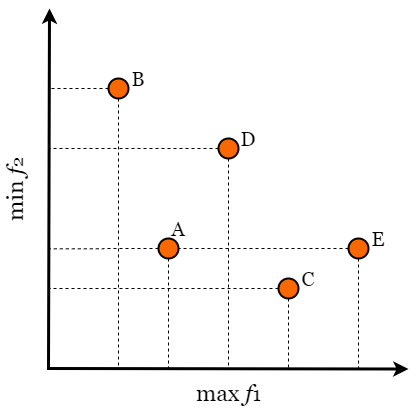
\includegraphics[scale=0.5]{images/pareto_dominance.png}
  \caption{
    Példa egy optimalizálási feladatra, ahol az $f_1$ célfüggvényt maximalizálni, míg az $f_2$ célfüggvényt minimalizálni kell.
  }
  \label{fig:PARETO_DOMINANCE}
\end{figure}


\subsection{Nash-dominancia}



\subsection{Berge-dominancia}
